\chapter{Implementaci\'{o}n de la aproximaci\'{o}n y Ofeli}

Una vez encontrada una t\'{e}cnica que contemplara los requisitos del proyecto, se empez\'{o} a buscar alguna implementaci\'{o}n sobre esta t\'{e}cnica. En esa b\'{u}squeda se encontr\'{o} un trabajo llamado Ofeli (\textit{Open, Fast and Efficient Level set Implementation}) \cite{ofeli}. Este trabajo est\'{a} desarrollado con Qt que es una de librer\'{i}as multiplataforma para la realizaci\'{o}n de aplicaciones con GUI (\textit{graphical user interface}) en C++. Esta aplicaci\'{o}n es muy completa ya que, aparte del algoritmo de inter\'{e}s, implementa varias funcionalidades extra como varios tipos de filtrado, preprocesamiento, varios tipos de evoluci\'{o}n del contorno, etc.

\section{Ofeli}

En esta secci\'{o}n se explicar\'{a} la estructura de la implementaci\'{o}n y las clases que se utilizan en este trabajo. Se realizar\'{a} un esquema general para que el lector pueda comprender cu\'{a}les son los procesos o pautas que se dan en esta implementaci\'{o}n para poder segmentar una imagen.


\subsection{Estructura}

La implementaci\'{o}n est\'{a} formada por varias clases que se han dividido en dos tipos: las clases o ficheros que pertenecen a la GUI (etiquetadas con la palabra <<GUI->> por delante de sus nombres) y las clases que pertenecen a la implementaci\'{o}n del algoritmo (etiquetadas con la palabra <<Impl->>).

\begin{enumerate}
	\item Impl-\textbf{ActiveContour}: clase padre de todos los tipos de contornos. Formada por lo ficheros:
		\begin{enumerate}
			\item activecontour.cpp
			\item activecontour.hpp
		\end{enumerate}
	\item Impl-\textbf{ACwithoutEdges}: clase que implementa el contorno que evolucionar\'{a} en una imagen a escala de grises. Formada por lo ficheros:
	\begin{enumerate}
		\item ac\_withoutedges.cpp
		\item ac\_withoutedges.hpp
	\end{enumerate}
	\item Impl-ACwithoutEdgesYUV: clase que implementa el contorno que evolucionar\'{a} en una imagen a color. Formada por lo ficheros:
	\begin{enumerate}
		\item ac\_withoutedges\_yuv.cpp
		\item ac\_withoutedges\_yuv.hpp
	\end{enumerate}
	\item Impl-\textbf{list}: implementaci\'{o}n de una lista ligada gen\'{e}rica. Formada por lo ficheros:
	\begin{enumerate}
		\item linked\_list.tpp
		\item linked\_list.hpp
	\end{enumerate}
	\item Impl-Filters: clase que implementa los filtros que se le pueden aplicar a la imagen antes de realizar la segmentaci\'{o}n. Formada por lo ficheros:
	\begin{enumerate}
		\item filters.cpp
		\item filters.hpp
	\end{enumerate}
	\item Impl-GeodesicAC: clase que implementa un contorno geod\'{e}sico. Formada por lo ficheros:
	\begin{enumerate}
		\item geodesic\_ac.cpp
		\item geodesic\_ac.hpp
	\end{enumerate}
	\item Impl-HausdorffDistance: clase que implementa la distancia de Hausdorff. Formada por lo ficheros:
	\begin{enumerate}
		\item hausdorff\_distance.cpp
		\item hausdorff\_distance.hpp
	\end{enumerate}
	\item GUI-ImageViewer: formada por los ficheros:
	\begin{enumerate}
		\item imageviewer.cpp
		\item imageviewer.hpp
	\end{enumerate}
	\item GUI-PixmapWidget: formada por los ficheros:
	\begin{enumerate}
		\item pixmapwidget.cpp
		\item pixmapwidget.hpp
	\end{enumerate}
\end{enumerate}
 
Se han resaltado las tres clases que interesar\'{a}n: \textit{ActiveContour}, \textit{ACwithoutEdges} y \textit{list}. Las dem\'{a}s clases a\~{n}aden funcionalidades extra que no son necesarias en este proyecto.
 
\subsection{Esquema general}

 \begin{figure}[H]
 	\captionsetup{justification=centering}
 	\centering
 	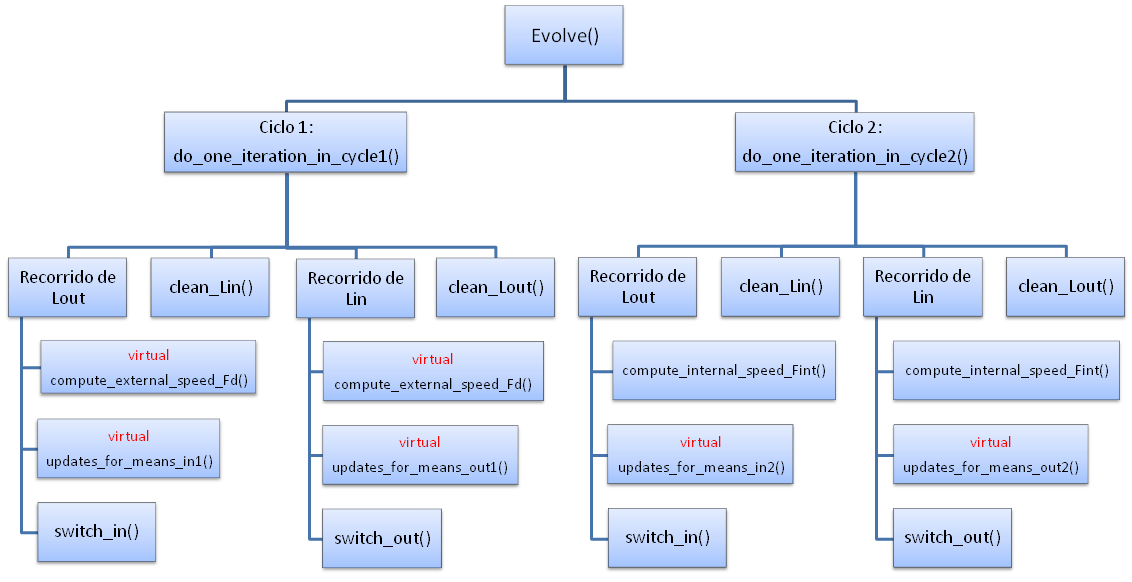
\includegraphics[width=1.3\textwidth]{./imagenes/esquemaOfeli}
 	\caption{Esquema de las funciones utilizadas en el trabajo de Ofeli para realizar el algoritmo \textit{level set }aproximado}	
 	\label{esquemaOfeli}
 \end{figure}

Como se puede observar la estructura del c\'{o}digo es pr\'{a}cticamente igual al algoritmo de aproximaci\'{o}n presentado en \ref{algoritmoFastLevelSet} exceptuando que en esta implementaci\'{o}n la velocidad de cada punto se calcula a la hora de tratar \'{e}ste, no se calculan todas las velocidades de todos los puntos a la vez como se sugiere en el algoritmo \ref{algoritmoFastLevelSet}. El c\'{a}lculo de estas velocidades son las funciones  \textit{compute\_(internal/external)\_speed\_($Fd/F_{int}$)} que se pueden ver en el esquema \ref{esquemaOfeli}. Las funciones  \textit{update\_for\_means\_(in/out)(1/2)} que no est\'{a}n en el algoritmo de aproximaci\'{o}n presentado en \ref{algoritmoFastLevelSet} se realizan para poder <<adaptar>> el contorno a la imagen de manera que \'{e}ste pueda evolucionar independientemente de los niveles de gris que se est\'{e}n utilizando en la imagen. Esto se refiere a que se va haciendo una media de las intensidades de los puntos pertenecientes a las listas que representan impl\'{i}citamente el contorno, es decir, $L_{out}$ y $L_{in}$, de manera que el umbral con el que se va decidiendo la velocidad de cada punto va cambiando en funci\'{o}n de los puntos que representan el contorno.

Las funciones definidas como \textit{clean()} son las limpiezas de las listas sobre puntos redundantes que pudiera haber que se nombra en el algoritmo \ref{algoritmoFastLevelSet}. Debe de quedar claro que estas funciones recorren las listas completamente al igual que la evoluci\'{o}n de cada una de ellas.

Otra cuesti\'{o}n a comentar es la etiqueta <<virtual>> que tienen varias funciones en el esquema \ref{esquemaOfeli} que significa exactamente, que la funci\'{o}n es virtual. Esta caracter\'{i}stica es importante a la hora de entender la jerarqu\'{i}a de las clases y con ello la estructura del trabajo Ofeli. Una funci\'{o}n virtual en el lenguaje de programaci\'{o}n C++ se utiliza en cuestiones de herencia y polimorfismo, de manera que clases hijas puedan redefinir funciones definidas como virtuales en la clase padre. As\'{i} pues, las funciones  \textit{compute\_external\_speed\_Fd} y \textit{update\_for\_means\_(in/out)(1/2)} est\'{a}n definidas con esta cl\'{a}usula ya que dependen de los datos, en este caso de las im\'{a}genes, y hay varias clases para trabajar con ellas en este trabajo. Si son im\'{a}genes a color se utilizar\'{a} la clase \textit{ACwithoutEdgesYUV}, mientras que si es una imagen a escala de grises se trabajar\'{a} con la clase \textit{ACwithoutEdges}, como se ha explicado en el anterior apartado.

Comentadas estas cuestiones se deduce que todas las funciones presentadas en el esquema \ref{esquemaOfeli} est\'{a}n implementadas en \textit{ActiveContour}, la clase padre, exceptuando aquellas que tienen la etiqueta <<virtual>> que las implementar\'{a}n las clases hijas \textit{ACwithoutEdges} y \textit{ACwithoutEdgesYUV} dependiendo de las caracter\'{i}sticas de la imagen.
 
Para finalizar, la implementaci\'{o}n de la lista ligada se utiliza para representar las listas $L_{out}$ y $L_{in}$ con las que estaremos trabajando continuamente en los dos ciclos.